%-----------------------------------------------------------------------------------------------------------------------------------------------%
%	The MIT License (MIT)
%
%	Copyright (c) 2021 Jitin Nair
%
%	Permission is hereby granted, free of charge, to any person obtaining a copy
%	of this software and associated documentation files (the "Software"), to deal
%	in the Software without restriction, including without limitation the rights
%	to use, copy, modify, merge, publish, distribute, sublicense, and/or sell
%	copies of the Software, and to permit persons to whom the Software is
%	furnished to do so, subject to the following conditions:
%	
%	THE SOFTWARE IS PROVIDED "AS IS", WITHOUT WARRANTY OF ANY KIND, EXPRESS OR
%	IMPLIED, INCLUDING BUT NOT LIMITED TO THE WARRANTIES OF MERCHANTABILITY,
%	FITNESS FOR A PARTICULAR PURPOSE AND NONINFRINGEMENT. IN NO EVENT SHALL THE
%	AUTHORS OR COPYRIGHT HOLDERS BE LIABLE FOR ANY CLAIM, DAMAGES OR OTHER
%	LIABILITY, WHETHER IN AN ACTION OF CONTRACT, TORT OR OTHERWISE, ARISING FROM,
%	OUT OF OR IN CONNECTION WITH THE SOFTWARE OR THE USE OR OTHER DEALINGS IN
%	THE SOFTWARE.
%	
%
%-----------------------------------------------------------------------------------------------------------------------------------------------%

%----------------------------------------------------------------------------------------
%	DOCUMENT DEFINITION
%----------------------------------------------------------------------------------------

% article class because we want to fully customize the page and not use a cv template

%%%% DEBUG COMMAND
%%%%\listfiles

\documentclass[a4paper,12pt]{article}
\usepackage[utf8]{inputenc}

%----------------------------------------------------------------------------------------
%	FONT
%----------------------------------------------------------------------------------------

% % fontspec allows you to use TTF/OTF fonts directly
% \usepackage{fontspec}
% \defaultfontfeatures{Ligatures=TeX}

% % modified for ShareLaTeX use
% \setmainfont[
% SmallCapsFont = Fontin-SmallCaps.otf,
% BoldFont = Fontin-Bold.otf,
% ItalicFont = Fontin-Italic.otf
% ]
% {Fontin.otf}

%----------------------------------------------------------------------------------------
%	PACKAGES
%----------------------------------------------------------------------------------------
\usepackage{url}
\usepackage{parskip} 	

%other packages for formatting
\RequirePackage{color}
\RequirePackage{graphicx}
\usepackage[usenames,dvipsnames]{xcolor}
\usepackage[scale=0.9]{geometry}

%tabularx environment
\usepackage{tabularx}

%for lists within experience section
\usepackage{enumitem}

% centered version of 'X' col. type
\newcolumntype{C}{>{\centering\arraybackslash}X} 

%to prevent spillover of tabular into next pages
\usepackage{supertabular}
\usepackage{tabularx}
\newlength{\fullcollw}
\setlength{\fullcollw}{0.47\textwidth}

%custom \section
\usepackage{titlesec}				
\usepackage{multicol}
\usepackage{multirow}

%CV Sections inspired by: 
%http://stefano.italians.nl/archives/26
\titleformat{\section}{\Large\scshape\raggedright}{}{0em}{}[\titlerule]
\titlespacing{\section}{0pt}{10pt}{10pt}

%\titleformat{\subsection}{}{}{}{}[\titlerule]
%\titlespacing{\subsection}{0pt}{10pt}{10pt}


%for publications
%\usepackage[style=authoryear,sorting=ynt, maxbibnames=2]{biblatex}
%\usepackage[style=authoryear,sorting=ydnt,maxbibnames=100]{biblatex}

\usepackage[%backend=biber,
        style=numeric,
        sorting=ydnt,
        maxbibnames=100,
        defernumbers=true,
%        dateabbrev=false, % abbrev month display
        alldates=long]{biblatex}







\defbibheading{subbibliography}[\refname]{\subsection{#1}}
\setcounter{secnumdepth}{0}



%% \usepackage[
%%   style=publist,
%%   maxnames=11,
%%   plnumbering=local,
%%   marginyear=true,
%% ]{biblatex}



%Setup hyperref package, and colours for links
\usepackage[unicode, draft=false]{hyperref}
\definecolor{linkcolour}{rgb}{0,0.2,0.6}
\hypersetup{colorlinks,breaklinks,urlcolor=linkcolour,linkcolor=linkcolour}

% replace full url with hyperlink and symbol
\DeclareFieldFormat{url}{\mkbibacro{URL}\addcolon\space\href{#1}{\faExternalLink*}}
\newcommand{\myurl}[1]{URL:~\href{#1}{\faExternalLink*}}


\addbibresource{david_doukhan_ina.bib}
\addbibresource{david_doukhan_older.bib}
\addbibresource{david_doukhan_itw.bib}
\setlength\bibitemsep{1em}

%for social icons
\usepackage{fontawesome5}

%debug page outer frames
%\usepackage{showframe}



%%% MYFILTER

\defbibcheck{nokeyword}{%
\iffieldundef{keywords}{}{\skipentry}}


\usepackage{tikz} 


%----------------------------------------------------------------------------------------
%	BEGIN DOCUMENT
%----------------------------------------------------------------------------------------
\begin{document}

% non-numbered pages
%\pagestyle{empty} 



%----------------------------------------------------------------------------------------
%	TITLE
%----------------------------------------------------------------------------------------

% \begin{tabularx}{\linewidth}{ @{}X X@{} }
% \huge{Your Name}\vspace{2pt} & \hfill \emoji{incoming-envelope} email@email.com \\
% \raisebox{-0.05\height}\faGithub\ username \ | \
% \raisebox{-0.00\height}\faLinkedin\ username \ | \ \raisebox{-0.05\height}\faGlobe \ mysite.com  & \hfill \emoji{calling} number
% \end{tabularx}

\begin{tabularx}{\linewidth}{@{} C @{}}
\Huge{David Doukhan, Ph.D.} \\[7.5pt]
\href{https://github.com/DavidDoukhan}{\raisebox{-0.05\height}\faGithub\ DavidDoukhan} \ $|$ \
\href{https://www.researchgate.net/profile/David-Doukhan}{\raisebox{-0.05\height}\faResearchgate\ David-Doukhan} \ $|$ \ 
\href{https://linkedin.com/in/david-doukhan}{\raisebox{-0.05\height}\faLinkedin\ david-doukhan} \ $|$ \ 
%\href{https://mysite.com}{\raisebox{-0.05\height}\faGlobe \ mysite.com} \ $|$ \

\href{https://twitter.com/doukhan_david}{\raisebox{-0.05\height}\faTwitter \ doukhan\_david} \ $|$ \ 
\href{mailto:david.doukhan@gmail.com}{\raisebox{-0.05\height}\faEnvelope \ david.doukhan@gmail.com} \ $|$ \ 
\href{tel:+33678789781}{\raisebox{-0.05\height}\faMobile \ +33.6.78.78.97.81} \\
\end{tabularx}

\begin{tikzpicture}[remember picture, overlay]
  \node [anchor=north east, inner ysep=15pt, inner xsep=30pt]  at (current page.north east)
     {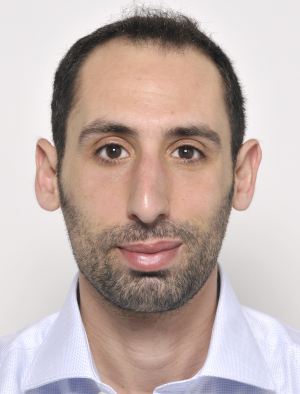
\includegraphics[height=3.2cm]{david_doukhan.jpg}};
\end{tikzpicture}

%\hfill
%\smash{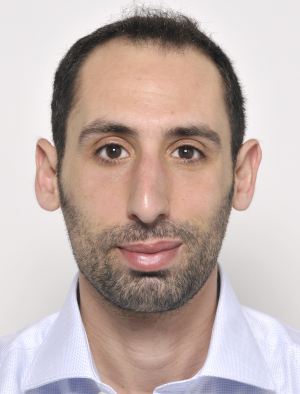
\includegraphics[width=2.5cm]{david_doukhan.jpg}}

%----------------------------------------------------------------------------------------
% EXPERIENCE SECTIONS
%----------------------------------------------------------------------------------------

%Interests/ Keywords/ Summary
\section*{Summary}

I'm researcher at \href{https://www.ina.fr}{Institut National de l'Audiovisuel (INA)} in Paris metropolitan area (France).
This document presents some elements of my CV together with my detailed publication and research dissemination list (last update: \today).
More information to come!
%My research interest range from audio analysis and synthesis (audio segmentation, speaker diarization and recognition, paralinguistics, prosodic analysis 3D audio, speech synthesis), 


\tableofcontents

%Experience
%% \section{Work Experience}

%% \begin{tabularx}{\linewidth}{ @{}l r@{} }
%% \textbf{Designation} & \hfill Jan 2021 - present \\[3.75pt]
%% \multicolumn{2}{@{}X@{}}{long long line of blah blah that will wrap when the table fills the column width long long line of blah blah that will wrap when the table fills the column width long long line of blah blah that will wrap when the table fills the column width long long line of blah blah that will wrap when the table fills the column width}  \\
%% \end{tabularx}

%% \begin{tabularx}{\linewidth}{ @{}l r@{} }
%% \textbf{Designation} & \hfill Mar 2019 - Jan 2021 \\[3.75pt]
%% \multicolumn{2}{@{}X@{}}{
%% \begin{minipage}[t]{\linewidth}
%%     \begin{itemize}[nosep,after=\strut, leftmargin=1em, itemsep=3pt]
%%         \item[--] long long line of blah blah that will wrap when the table fills the column width
%%         \item[--] again, long long line of blah blah that will wrap when the table fills the column width but this time even more long long line of blah blah. again, long long line of blah blah that will wrap when the table fills the column width but this time even more long long line of blah blah
%%     \end{itemize}
%%     \end{minipage}
%% }
%% \end{tabularx}

%% %Projects
%% \section{Projects}

%% \begin{tabularx}{\linewidth}{ @{}l r@{} }
%% \textbf{Some Project} & \hfill \href{https://some-link.com}{Link to Demo} \\[3.75pt]
%% \multicolumn{2}{@{}X@{}}{long long line of blah blah that will wrap when the table fills the column width long long line of blah blah that will wrap when the table fills the column width long long line of blah blah that will wrap when the table fills the column width long long line of blah blah that will wrap when the table fills the column width}  \\
%% \end{tabularx}

%% %----------------------------------------------------------------------------------------
%% %	EDUCATION
%% %----------------------------------------------------------------------------------------
\section{Education}
\begin{tabularx}{\linewidth}{@{}l X@{}}	
2009-2013 & Ph.D. in Computer Science under the supervision of Christophe D’Alessandro (LIMSI-CNRS) and Albert Rilliard (LIMSI-CNRS), Paris Sud University.\\
2008-2009 & Master of Sciences ATIAM (Acoustics, Signal Processing and Computer Sciences applied to Music) co-hosted by University Pierre et Marie Curie (Paris VI), IRCAM, and Telecom Paris.\\
2005 & Student Exchange Program in Indian Institute of Technology Kanpur (India). Validated courses: Indian Art And Civilization, Machine Learning, Signal Processing, Mathematics\\
2001-2007 & EPITA (School of Engineering and Computer Science), major Artificial Intelligence and Machine Learning (SCIA). Graduated with honours (mention bien)\\
2001 & Scientist Baccalaureat (A-level), major physic\\
\end{tabularx}



\section{Editorial, Animation and Evaluation activities}
\subsection{Scientific Animation}
\begin{enumerate}
\item Music Information Retrieval Evaluation eXchange (MIREX - 2018). Task Captain in change of voice and music activity detection challenge in collaboration with Blai Meléndez-Catalán (BMAT/UPF) \myurl{https://www.music-ir.org/mirex/wiki/2018:Music_and/or_Speech_Detection}.
\item Journées d’étude et de Formation sur la Parole (JEFP - 2012). Member of the organization committee
\end{enumerate}
\subsection{Journal and conference reviewing committee}
\begin{enumerate}
\item revue TAL \myurl{https://www.atala.org/node/16}
\item The Journal of the Acoustical Society of America (JASA)
\item EURASIP Journal on Audio, Speech, and Music Processing
\item Frontiers in Computer Science
\item Annual Conference of the International Speech Communication Association (INTERSPEECH - ISCA)
\item International Conference on Acoustics, Speech, and Signal Processing (IEEE ICASSP)
\item International Conference on Language Resources and Evaluation (LREC)
\item Phonetics and Phonology in Europe (Pape)
\item Journées d’Etudes de la Parole (JEP - AFCP)
\end{enumerate}
\subsection{Funded Project Evaluation}
\begin{enumerate}
\item Member of International Federation of Television Archives (IFTA) Media Studies Grant Commission (2020-2021)
\item Member of French National Research Agency (ANR) CE38 evaluation committee (2018)
\end{enumerate}







%----------------------------------------------------------------------------------------
%	PUBLICATIONS
%----------------------------------------------------------------------------------------
\section{Publications and Research Dissemination}
\begin{refsection}[david_doukhan_ina.bib,david_doukhan_older.bib,david_doukhan_itw.bib]
\nocite{*}
\printbibliography[type=article, check=nokeyword, heading=subbibliography, title={Peer-reviewed journal papers}, resetnumbers=true]
\printbibliography[type=inproceedings, check=nokeyword, heading=subbibliography, title={Peer-reviewed conference proceedings}, resetnumbers=true]
\printbibliography[type=inproceedings, keyword={abstract}, heading=subbibliography, title={Peer-reviewed abstract papers}, resetnumbers=true]
\printbibliography[type=thesis, heading=subbibliography, title={PhD Thesis}, resetnumbers=true]
\printbibliography[type=report, heading=subbibliography, title={Governmental and non-governmental reports on women and diversity representation in media (contributions)}, resetnumbers=true]
\printbibliography[type=article, heading=subbibliography, keyword={general}, title={General audience and science popularization articles}, resetnumbers=true]
\printbibliography[type=unpublished, keyword={invit}, heading=subbibliography, title={Invited Speaker}, resetnumbers=true]
\printbibliography[type=inproceedings, keyword={publicaudition}, heading=subbibliography, title={Public auditions and scientific expertise}, resetnumbers=true]
\printbibliography[keyword={itw}, heading=subbibliography, title={Interventions and interviews in general audience media (press, audiovisual, pure players)}, resetnumbers=true]
\end{refsection}

%----------------------------------------------------------------------------------------
%	SKILLS
%----------------------------------------------------------------------------------------


%% \section{Skills}
%% \begin{tabularx}{\linewidth}{@{}l X@{}}
%% Some Skills &  \normalsize{This, That, Some of this and that etc.}\\
%% Some More Skills  &  \normalsize{Also some more of this, Some more that, And some of this and that etc.}\\  
%% \end{tabularx}

%% \vfill


\end{document}
